% !TeX root = surgery.tex
\subsection{The Nepalese Version}
Andrey's contribution here

\subsection{Cakrapāṇidatta and Ḍalhaṇa's Versions}
The commentaries of Cakrapāṇidatta and Ḍalhaṇa, called the \emph{Bhānumatī} and \emph{Nibandhasaṅgraha} respectively, are based on similar versions of the \SS, both of which are significantly different to the Nepalese version. Ḍalhaṇa was aware of Cakrapāṇidatta's work and reiterated many of his predecessor's remarks, so the commentator's interpretation of the root text is largely consistent. 

Trikamajī Ācārya's edition of the \textit{Sūtrasthāna} of the \emph{Bhānumatī} \citep{acar-1939} duplicates the version of the \SS\ in his edition of the \emph{Nibandhasaṅgraha} \citep{vulgate}, except in a few obvious cases where Cakrapāṇidatta glosses a word or compound that is different to the one glossed by Ḍalhaṇa.\footnote{For example, in SS.1.16.18, Cakrapāṇidatta glosses \emph{rājasarṣapa} whereas Ḍalhaṇa glosses \emph{gaurasarṣapa}, and Ācārya reflects this in the root texts of the \emph{Bhānumatī} \citep[130]{acar-1939} and \emph{Nibandhasaṅgraha} \citep[79]{vulgate}.} The duplication of the root text creates the somewhat misleading impression that both commentators had an almost identical version of the \SS. However, there is evidence in SS.1.16 that this was not the case. For example, Ḍalhaṇa comments on four verses (1.16.11–14, \cite[78]{vulgate}) that Cakrapāṇidatta cites separately in his commentary \citep[128–129]{acar-1939}, introducing each one as 'some people read' (\emph{ke cit paṭhanti}). This clearly indicates that these verses were not in the version of the \SS\ upon which Cakrapāṇidatta was commenting, yet Ācārya includes them in the root text of the \emph{Bhānumatī}.

Also, Cakrapāṇidatta does not acknowledge or comment on some verses in the version of the \SS\ known to Ḍalhaṇa. Although it is possible that a commentator may not have remarked on a verse because its meaning was clear, in some cases the commentarial convention of citing the first words of a new verse or passage provides firmer ground for suspecting the absence of a verse in the root text. For example, the prose passage of SS.1.16.18 in the the \emph{Bhānumatī} \citep[130]{acar-1939}, which is SS.1.16.19 in the \emph{Nibandhasaṅgraha} \citep[79]{vulgate}, is followed by several verses that elaborate on the content of the prose passage, and both commentators introduce these verses and cite the opening words of the first verse before glossing specific terms. However, Cakrapāṇidatta does not introduce, cite or comment on the same verses as Ḍalhaṇa (SS.1.16.20–22ab, \cite[79]{vulgate}), and yet the first of the verses commented on by Ḍalhaṇa appears in the root text of Ācārya's edition of the \emph{Bhānumatī} (SS.1.16.19, \cite[130]{acar-1939}), and the others (SS.1.16.20–21ab) are included in parenthesis. A similar instance of this occurs at \emph{Bhānumatī} SS.1.16.31, where Ācārya includes a verse in parenthesis that was commented on by Ḍalhaṇa (SS.1.16.32, \cite[81]{vulgate}) but not by Cakrapāṇidatta. It appears that the manuscript on which Ācārya's edition of the \emph{Bhānumatī} was based does not include the root text.\footnote{This observation is based on the opening passage of MS 1887-1935 of the \emph{Bhānumatī}, which is transcribed in Eggling 1896: 928. The transcription has the commentary without the root text. See the section below on Ācārya's 1939 edition for details of the sources Ācārya used for this edition.} Therefore, the inclusion of SS.1.16.19–21ab and 31 in the root text of the \emph{Bhānumatī} is an unsubstantiated hypothesis. 

% Ḍalhaṇa 1.16.11–14
%The version of 1.16.11–14 known to Ḍalhaṇa \citep[78]{vulgate} has four verses (\emph{śloka}) at this point that are not in the Nepalese manuscripts. The additional verses iterate the types of joins required for ear flaps that are missing, elongated, thick, wide, etc. All four verses were probably absent in the version of the \emph{Suśrutasaṃhitā} known to Cakrapāṇidatta. He cites the verses separately in his commentary, the \emph{Bhānumatī} \citep[128–129]{acar-1939}, introducing each one as 'some people read' (\emph{ke cit paṭhanti}). However,  in Trikamajī Ācārya's edition of the \emph{Sūtrasthāna} of the \emph{Bhānumatī}, the root text is largely identical to the one commented on by Ḍalhaṇa (\cite{vulgate}), even in instances like this where Cakrapāṇidatta's commentary indicates that he was reading a different version of the \emph{Suśrutasaṃhitā}

% Ḍalhaṇa 1.16.19–20 
%Cakrapāṇidatta \citep[131]{acar-1939} does not comment on these verses, nor verse 15 of the Nepalese version, and so the version of the \emph{Suśrutasaṃhitā} known to him may not have included them.

% Ḍalhaṇa 1.16.32
 %Cakrapāṇidatta \citep[133]{acar-1939} does not comment on this additional verse, which suggests that either he did not know of it or was not inclined to accept it.
 
% Both commentators were aware of a version of the \SS\ that was similar to the Nepalese version % See blog.

In fact, there is some evidence that the Nepalese version was more similar to Cakrapāṇidatta's version than to Ḍalhaṇa's. For example, 1.16.5 of the Nepalese version begins with the compound \emph{doṣasamudayāt} whereas the version known to Ḍalhaṇa (SS.1.16.6, \cite[77]{vulgate}) inserts two compounds, \emph{kliṣṭajihmāpraśastasūcīvyadhāt} and \emph{gāḍhataravartitvāt}, before this. Cakrapāṇidatta (SS.1.16.5, \cite[126–127]{acar-1939}) begins his comment on this passage by glossing \emph{doṣasamudayāt}, which suggests that he was not aware of any compounds prior to this one. If one looks beyond SS.1.16, there are instances where the Nepalese version (1.1.28) and the root text of Cakrapāṇidatta have the same reading, which Ḍalhaṇa mentions as an alternative read by others. For example, 1.1.28 of the Nepalese version has \emph{tatrāsmiñ chāstre}, which is the reading commented on by Cakrapāṇidatta (\cite[17]{acar-1939}). However, Ḍalhaṇa  (SS.1.1.22, \cite[5]{vulgate}) comments on \emph{asmiñ chāstre} and states that others read \emph{tatrāsmiñ chāstre}. Also, in his commentary on SS.1.1.8.1, Ḍalhaṇa (\cite[5]{vulgate}) notes the variant reading \emph{ṣaṣṭyā vidhānaiḥ}, which is not in his root text but evidently was in Cakrapāṇidatta's  (SS.1.1.6, \cite[11]{acar-1939}). As discussed elsewhere (Birch 2021), the reading of \emph{ṣaṣṭyā vidhānaiḥ} is likely a corruption of \emph{ṣaṣṭyābhidhānaiḥ} in the Nepalese version (1.1.9). 




 
% Ḍalhaṇa was aware of the reading in the Nepalese version because he notes in his commentary on 1.16.6 \citep[77]{vulgate} that some read 'because of the accummulation of humours' rather than 'because of piercing with a painful, crooked and unrecommended needle or because of a wick that is too thick.' 

\subsection{Differences between the Nepalese and Subsequent Versions of SS.1.16}

The structural differences between the Nepalese and subsequent versions has been discussed by \citet[27–44]{kleb-2021b}, which include the frame story,\footnote{On this topic, also see the more recent \citet{birc-2021}.} the name of the first book (\emph{Ślokasthāna}), the structuring of the text according to chapter and section colophons, and an additional passage in the \emph{Kalpasthāna}. \citet[44–55]{kleb-2021b} also makes general observations on distinct features of the Nepalese version's content and looks specifically at lists of skin lesions arising from urinary disease and vital energies. And in an effort to demonstrate the possibility of greater coherence in the Nepalese version, \citet[101–104]{hari-2011} has compared its classification of snakes with Ḍalhaṇa's version. 

On the whole, these observations indicate that [...synopsis of general conclusions here, Andrey?...]
% 1.16 is missing yathovāca bhagavān dhanvantariḥ|

The following detailed comparison of 1.16 of the Nepalese version with Ḍalhaṇa's \emph{Nibandhasaṅgraha} unfolded as the chapter was edited. The differences appear to emanate largely from attempts to standardise, simplify or clarify the language of the Nepalese version, add and redact information, and introduce changes to recipes and treatments. Examples from 1.16 have been provided to demonstrate the general observations which, it is hoped, a larger survey of the text will verify.

Table 1 reveals the extent to which 1.16 of the Nepalese version was redacted to create the one known by Ḍalhaṇa. In this particular case, twenty-seven verses have been added, eight (11-14, 21–22ab, 23cd–24, 32) of which are well-integrated with the existing material in so far as they reiterate and elaborate on the content of passages in the Nepalese version. A block of nineteen verses (26.1–19) at the end of this chapter in Ācārya's edition of the \emph{Nibandhasaṅgraha} (\cite[80]{vulgate}) was known by Ḍalhaṇa. These verses cover additional diseases of the ear lobes, as well as their treatment and complications. Although Ḍalhaṇa concedes that some read them in this chapter, he concludes that they were not composed by sages and, therefore, should not be read. Ācārya probably included these verses because they were in his manuscripts,\footnote{Ācārya does not state that these verses were absent in some or all of his manuscripts, which he usually does in a footnote if this is the case. A broader survey of manuscripts would be helpful for establishing whether these verses were part of the transmission of the \SS\ in India. For example, they are in MS Hyderabad Osmania 137-3(b).} and Ḍalhaṇa's comments prompted him to place them in parentheses. Be this as it may, this large block of verses is absent in the Nepalese version. 

\begin{table}
\centering
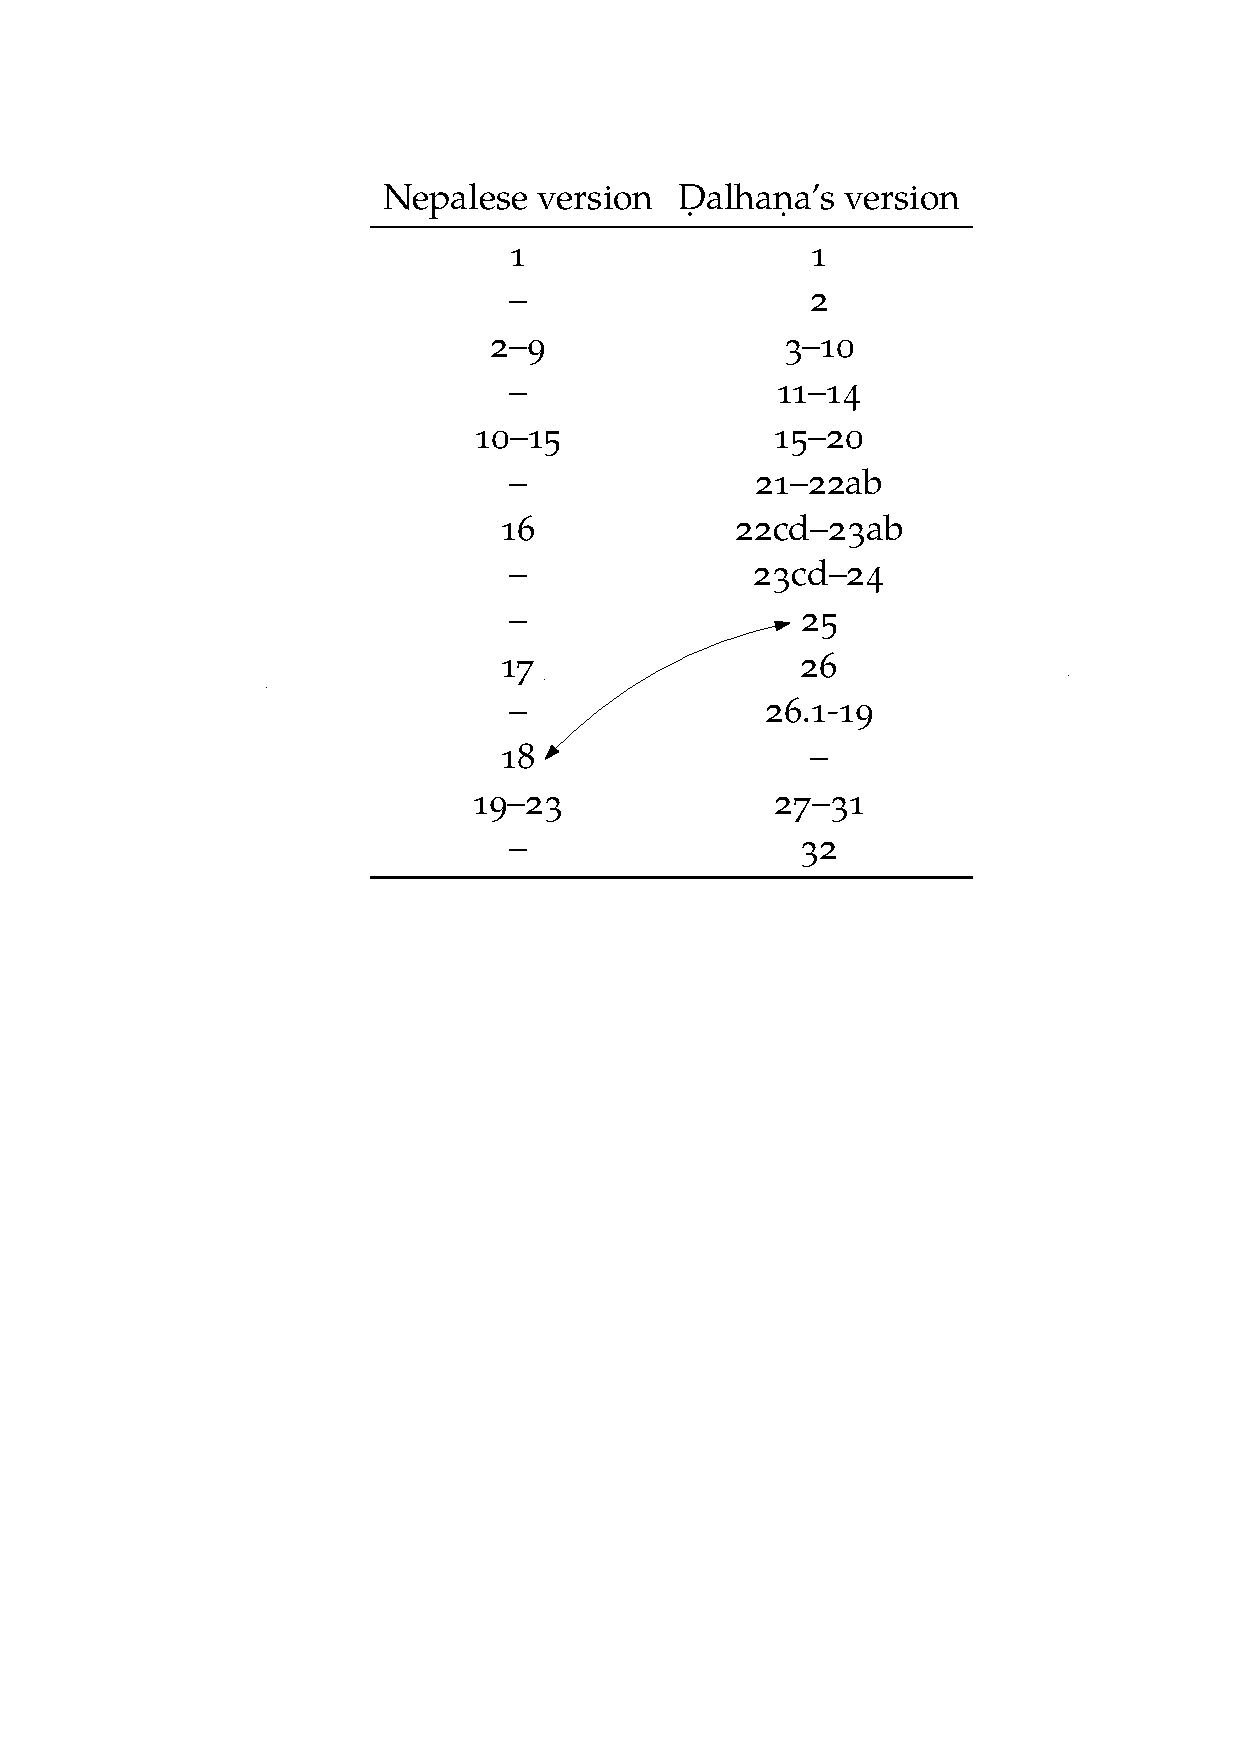
\includegraphics[draft=false,width=\textwidth]{table-of-versions.pdf}
\caption{A Comparison of Verses in 1.16 of the Nepalese and Ḍalhaṇa's Versions}
\end{table}

In Table 1, one can also see that verses 17 and 18 of the Nepalese version were transposed in the redaction of Ḍalhaṇa's version, in which they are 26 and 25 respectively. Although this only occurs once in 1.16, such transposing of verses and even their hemistiches is more prevalent in the redaction of other chapters of the \SS.

Apart from the addition of verses, the redacting of the version known to Ḍalhaṇa involved many small, yet sometimes significant, changes that are summarised below. 

\subsubsection{Changing Spelling, Sandhi and Syntax}
In the majority of cases, efforts were made by redactors to standardise, simplify or improve the language of the Nepalese version. Such changes include the standardising of spelling,\footnote{For example, \emph{pattāṅga} (SS.1.16.21) → \emph{pataṅga} (1.16.29, \cite[81]{vulgate}). For more information on this, see the relevant footnote to the translation.} sandhi,\footnote{or example, \emph{°hastena ṛju} (SS.1.16.2) → \emph{°hastena rju} (1.16.3, \cite[76]{vulgate}).} and verbal forms,\footnote{For example, \emph{unnāmayitvā} (SS.1.16.21) → \emph{prānnamya} (1.16.29, \cite[81]{vulgate}); \emph{avacūrṇayīta} (SS.1.16.21) → \emph{upaharet} (1.16.29, \cite[81]{vulgate}).} as well as interventions to simplify and clarify syntax,\footnote{For example, \emph{śoṇitabahutvanivedanāyāṃ cānyadeśaviddham iti jānīyāt | nirupadravatā taddeśaviddhaliṅgam |} (SS.1.16.3) → \emph{śoṇitabahutvena vedanayā cānyadeśaviddham iti jānīyāt | nirupadravatayā taddeśaviddham iti |} (1.16.4, \cite[76]{vulgate}); \emph{āmatailapariṣekeṇopacaret} (SS.1.16.6) → \emph{āmatailena pariṣecayet} (1.16.7, \cite[77]{vulgate}); \emph{suparigṛhītaṃ} (SS.1.16.10) → \emph{suparigṛhītaṃ ca kṛtvā} (1.16.15, \cite[78]{vulgate}); \emph{anena} (SS.1.16.15) → \emph{snehenaitena} (1.16.20, \cite[79]{vulgate}).} which often involved splitting compounds.\footnote{For example, \emph{yadṛcchāviddhāyāṃ sirāyām} (SS.1.16.4) → \emph{yadṛcchayā viddhāsu	sirāsu} (1.16.5, \cite[76]{vulgate}); \emph{dhānyāmlakapālacūrṇaṃ} (SS.1.16.10) → \emph{dhānyāmlaṃ kapālacūrṇaṃ} (1.16.20, \cite[78]{vulgate}).} In some instances, these changes improved the grammar,\footnote{For example, \emph{surāmaṇḍakṣīram} (SS.1.16.10) → \emph{surāmaṇḍaṃ kṣīram} (1.16.15, \cite[78]{vulgate}).} or altered the meaning.\footnote{For example, \emph{kṣīṇālpamāṃsaḥ} (SS.1.16.12) → \emph{kṣīṇo 'lpamāṃsaḥ} (1.16.17, \cite[79]{vulgate}).} However, some prefixes of verbal forms,\footnote{For example, \emph{samvarddhitaḥ} (SS.1.16.8) → \emph{vivarddhitaḥ} (1.16.9, \cite[77]{vulgate}); \emph{niveśya} (SS.1.16.10) → \emph{sanniveśya} (1.16.15, \cite[78]{vulgate}); \emph{avabadhya} (SS.1.16.10) → \emph{ca baddhvā} (1.16.15, \cite[78]{vulgate}).} case endings,\footnote{For example, \emph{māse} (SS.1.16.2) → \emph{māsi} (1.16.3, \cite[76]{vulgate}).} and indeclinables were changed for less apparent reasons.\footnote{For example, \emph{api} (SS.1.16.13) → \emph{vā} (1.16.18, \cite[79]{vulgate}); \emph{ca} (SS.1.16.16) → \emph{tu} (1.16.23, \cite[79]{vulgate}); \emph{tu} (SS.1.16.18) → \emph{ca} (1.16.25, \cite[80]{vulgate}).} There is also a tendency to replace uncommon words with generic ones,\footnote{For example, \emph{mrakṣayet} (SS.1.16.15) → \emph{yojayet} (1.16.20, \cite[79]{vulgate}); \emph{nahyet} (SS.1.16.21) → \emph{baddhvā} (1.16.29, \cite[81]{vulgate}).} add indeclinables,\footnote{For example, [absent]  (SS.1.16.6) → \emph{ca} (1.16.7, \cite[77]{vulgate}); [absent] (SS.1.16.10) → \emph{tatra} (1.16.15, \cite[78]{vulgate}); [absent]  (SS.1.16.12) → \emph{api} (1.16.17, \cite[79]{vulgate}).} omit the verb to be at the end of sentences,\footnote{The words \emph{bhavati} or \emph{bhavanti} are omitted four times in Ḍalhaṇa's version (1.16.10 (twice), 1.16.17 and 1.16.18, \cite[77, 79]{vulgate}).}and introduce verses after a prose passage with the phrase \emph{bhavati cātra}.\footnote{For example, [absent] (SS.1.16.11) → \emph{bhavati cātra} (1.16.16, \cite[79]{vulgate}).} 

% Spelling
% 9. nemī → nemi
% 9. yaṣṭī → yaṣṭi
% 9. kākauṣṭhaḥ → kākauṣṭhakaḥ
% 21. pattāṅga → pataṅga *

%Sandhi
% 2 °hastena ṛju  →  °hastena rju (standardise)*

% Standardising and Simplifying Syntax
% 3.  śoṇitabahutvanivedanāyāṃ cānyadeśaviddham iti jānīyāt | nirupadravatā taddeśaviddhaliṅgam || → śoṇitabahutvena vedanayā cānyadeśaviddham iti jānīyāt || nirupadravatayā taddeśaviddham iti ||*
% 6 āmatailapariṣekeṇopacaret → āmatailena pariṣecayet*

% Clarifying syntax
%15 anena → snehenaitena*

% Splitting compounds
% 4. yadṛcchāviddhāyāṃ	sirāyām	 → 	yadṛcchayā viddhāsu	sirāsu (clarifies syntax)*
% 10. surāmaṇḍakṣīram → surāmaṇḍaṃ kṣīram (improves grammar)*
% 10. dhānyāmlakapālacūrṇañ → dhānyāmlaṃ kapālacūrṇañ*
% 12. kṣīṇālpamāṃsaḥ → kṣīṇo 'lpamāṃsaḥ (changes the meaning)*

% Changing verbs and gerunds
% 2. vyadhayet → vidhyete (perhaps, picking up on karnau)
% 6. kurvīta → dadyāt (middle to active) 
% 7. muñcet → kuryāt
% 9. bandhyā bhavanti → sādhyāḥ
% 10. suparigṛhītaṃ → suparigṛhītaṃ ca kṛtvā ( attempt to improve syntax)*
% 10. upapādya → upadhārya
% 10. sandarśya → sandadhyāt | tato (attempt to simplify the sentence)
% 13. chidyeta → chidyate (opt to pres)
% 15. mrakṣayet → yojayet * (replacing less common words with generic ones)
% 21. nahyet → baddhvā*
% 21. unnāmayitvā → prānnamya (standardise)*
%21 avacūrṇayīta → avacūrṇayet (standardise)*

% Omitting bhavati
% Happens a few times; e.g., 1.16.9 (twice), 1.16.12, 1.16.13

% Changing Prefixes
% 8. samvarddhitaḥ → vivarddhitaḥ*
% 10. niveśya → sanniveśya*
% 10. avabadhya → ca baddhvā*
% 15. marditaṃ → unmarditaṃ*
% 21. unnāmayitvā → prānnamya *

% Changing case endings
% 2. māse → māsi (shift from māsa to mās. Can't see a reason)
% 3. śoṇitabahutvanivedanāyāṃ →  śoṇitabahutvena vedanayā (splitting compounds, but locative of circumstance or condition changed to instrumental of reason. latter is clearer, but not much in it)
% 19. viśleṣitāyām atha nāsikāyāṃ → °tāyās tv nāsikāyāḥ

% changing indeclinables
%13 anyathā → ato 'nyathā
% 13 api → vā*
% 15 tataḥ → ataḥ
% 16 ca → tu*
% 18 tu → ca*
% 19 atha → tu
% 23 vai → syāt

% Adding indeclinables
% 10 [absent] → tatra
% 6 [absent] → ca
% 9 [absent] → tu
% 10 [absent] → ca
% 12 [absent] → api
% 14 [absent] → vā

% Omitting indeclinables
% 9 tatra → [absent]
% 9 ca → [absent]

%Adding bhavati cātra before verses.

% Not sure
% 2
% kṛtamaṅgalaṃ svastivācanan → kṛtamaṅgalasvastivācanan (the latter makes better sense, but could have been original, in my opinion, or an attempt to better integrate a gloss that had become part of the text.)
% abhisāntvayamānaḥ → abhisāntvayan (shift from Pres Pass Part to Pres Act Part) % It seems only the latter is correct in the given context. So, it could be just an error in the NV. Emend or Change translation!!! 
% % 10. agropaharaṇīyāt appears to be an error in the NV that needs to be emended.

\subsubsection{Changing Technical Terms}
There is evidence of standardising and altering technical terminology in subsequent versions of the \SS. Two examples of this in SS.1.16 are the terms for \se{bandha}{joins} and \se{vadhra}{a slice of flesh}. The Nepalese version uses three terms for \se{bandha, sandhāna, sandhi}{joining} splits in the ear flaps and the flesh of nose. Redactors of subsequent versions appear to have tried to standardise this terminology by replacing \emph{sandhāna} and \emph{sandhi} with \emph{bandha} in prose passages.\footnote{For example, \emph{pañcadaśasandhānākṛtayaḥ} (SS.1.16.9) → \emph{pañcadaśabandhākṛtayaḥ} (SS.1.16.10, \cite[77]{vulgate}); \emph{daśakarṇasandhivikalpāḥ} (SS.1.16.9) → \emph{karṇabandhavikalpāḥ} (SS.1.16.10, \cite[77]{vulgate})} However, the use of the term \emph{sandhāna} was retained in verses, perhaps because of the metrical challenges of making such a change. Also, the names of joins which incorporate \emph{sandhāna} and \emph{sandhi} remained the same.\footnote{These names are \emph{nemīsandhānaka}, \emph{kapāṭasandhika}, and \emph{ardhakapāṭasandhika} in SS.1.16.9.}

The Nepalese version (SS.1.16.20,23) contains the rather obscure term \emph{vadhra} for the slice of flesh that a surgeon cuts from the cheek in order to construct a new nose. Modern dictionaries define \emph{vadhra} as a leathern strap (\cite[1385]{apte-prac}, \cite[917]{Monier-Williams}) or a slice of bacon (\cite[917]{Monier-Williams}), the latter of which is more indicative of its meaning in the Nepalese version. This word was written out of subsequent verses,\footnote{\emph{vadhram} (SS.1.16.20) → \emph{baddham} (SS.1.16.28, \cite[81]{vulgate}) and \emph{tadvadhraśeṣaṃ} (SS.1.16.23) → \emph{tad ardhaśeṣaṃ} (SS.1.16.31, \cite[81]{vulgate}).} and it was not mentioned as an alternative reading by either Cakrapāṇidatta or Ḍalhaṇa, which suggests that its use and meaning may not have been known to them. However, \emph{vadhra} was used by the author of the \emph{Aṣṭāṅgahṛdayasaṃhitā} (\Ah{Utt.18.62}{841}) in the context of rhinoplasty, so it likely to be the correct reading in the Nepalese version. 

% bandha
% 1. athātaḥ karṇavyadhavidhim vyākhyāsyāmaḥ  → athātaḥ karṇavyadhabandhavidhim adhyāyaṃ (prose)
% sandhāna in all version (verse)
% 9. pañcadaśasandhānākṛtayaḥ (SS.1.16.9) → pañcadaśabandhākṛtayaḥ (SS.1.16.10) (sandhāna is reflected in the name nemisandhānaka, which is in all versions) 
% 9. daśakarṇasandhivikalpāḥ → karṇabandhavikalpāḥ (sandhi is in many of the names, bandha is not)
% 10. (twice) bandha in all versions
% 17 karṇabandha in all versions
% 19 & 23. sandhāna accepted in all versions + 32 in DV. (verse)
% 20. sādhubaddham → sādhubandhaiḥ (verse)
%
% vadhra 
% 20 vadhram → baddham 
% 21 susīvitaṃ → susaṃhitaṃ
% 23 tadvadhraśeṣaṃ → tad ardhaśeṣaṃ

\subsubsection{Augmenting the Text}

Apart from adding whole passages and verses (as seen in Table 1), redactors of subsequent versions augmented the text by expanding existing compounds and inserting new compounds and words. Within the microcosm of 1.16, adjectives and adverbs were inserted to clarify statements,\footnote{For example, \emph{chidre} (SS.1.16.2) → \emph{chidra ādityakarāvabhāsite} (1.16.3, \cite[76]{vulgate}); [absent] (SS.1.16.2) → \emph{śanaiḥ śanaiḥ} (1.16.3, \cite[76]{vulgate});  [absent] (SS.1.16.3) → \emph{āśu} (1.16.5, \cite[77]{vulgate}).} and phrases added to elaborate on diseases and treatments.\footnote{For example, \emph{dhātryaṅke} (SS.1.16.2) → \emph{dhātryaṅke kumāradharāṅke vā} (1.16.3, \cite[76]{vulgate}); [absent] (SS.1.16.2) → \emph{bālakrīḍanakaiḥ pralobhya} (1.16.3, \cite[76]{vulgate});  [absent] (SS.1.16.3) → \emph{picuvartiṃ praveśayet} (1.16.5, \cite[77]{vulgate}).} In particular, the characteristics and number of symptoms of a disease tend to increase in subsequent versions and models of classifying them were introduced. For example, the symptoms associated with incurable joins burgeoned from a list of four in the Nepalese version (SS.1.16.19) to six in Ḍalhaṇa's version (1.16.10, \cite[77]{vulgate}), reasons?


and the latter (1.16.5, \cite[76–77]{vulgate}) classifies the symptoms of mistakenly piercing a duct in the ear according to three ducts called \emph{kālikā}, \emph{marmarikā} and \emph{lohitikā}, which results in some repetition of the symptoms mentioned.\footnote{In the version known to Ḍalhaṇa  (1.16.5, \cite[76–77]{vulgate}), the symptoms of \se{jvara}{fever} and \se{vedanā}{pain} are repeated. This repetition does not occur in the Nepalese version.}

% Supplementary compounds and phrases for Adding Information
% This is done by expanding compounds, inserting new compounds and adverbs and adding verses and passages.
% 
% 1. karṇavyadhavidhim → karṇavyadhabandhavidhim (foregrounding the term bandha)
% 2
% dhātryaṅke → dhātryaṅke kumāradharāṅke vā (elaborating on treatment)
% upaveśyābhisāntvayamānaḥ → upaveśya bālakrīḍanakaiḥ pralobhyābhisāntvayan (elaborating on treatment)
% chidre → chidra ādityakarāvabhāsite (clarifying technical term)
% [absent] → śanaiḥ śanaiḥ (clarifying treatment)
% [absent] → picuvartiṃ praveśayet (elaborating on treatment)
% 4 
% [absent] →  kālikāmarmarikālohitikāsūpadravā and dividing the adverse affects according to kālikā, marmarikā and lohitikā. Repetition of vedanā and jvara in this process.(discussed in footnote). teṣu yathāsvaṃ pratikurvīt || (adding symptoms, perhaps with a view to managing them more effectively, according to the type of vein pierced).
% 5
% [absent] → kliṣṭajihmāpraśastasūcīvyadhād gāḍhataravartitvād (adding reasons)
% [absent] → yatra saṃrambho vedanā vā bhavati (adding information about the treatment)
%  [absent]  → āśu (clarifies the treatment)
%  [absent] → tāvad yāvat surūḍha iti (until it is well healed - clarifies the treatment)
%9
% pīṭhopamapālir nirvedhimaḥ → pīṭhopamapālir ubhayataḥ kṣīṇaputrikāśrito nirvedhimaḥ (adding characteristics)
% itarālpapāliḥ saṃkṣiptaḥ → utsannapālir itarālpapāliḥ saṃkṣiptaḥ (adding characteristics)
% tanuviṣamapālir → tanuviṣamālpapālir (adding characteristics)
% baddheṣv api dāhapākasrāvaśophayuktā	na siddhim upayānti → tu śophadāharāgapākapiḍakāsrāvayuktā	na siddhim upayānti (adding symptoms)
% 10
% surāmaṇḍodakābhyāṃ → surāmaṇḍoṣṇodakābhyāṃ (adding characteristics of an ingredient)
% 12
% gāḍhapākarāgavān → dāhapākarāgavedanāvān (adding symptoms)

% Additional Verses and Passages (table 1)
% For passages, see subsub on Elaborating on Treatments.
%  [absent] → 16.11–14 (verses)
%  [absent] → 21–22ab, 23cd–24
%  [absent] → 26.1 – 26.19
%  [absent] → 32

\subsubsection{Transposing Words, Verses and Passages}
% Words
% 9. aṇusthūla° → sthūlāṇu°
% 9. tatraite daśakarṇa° → tatra daśaite karṇa°
%  10. nātigāḍhan nātiśithilaṃ sūtreṇāvabadhya → sūtreṇānavagāḍhaman atiśithilaṃ ca baddhvā
% Passages
% 2. pūrvan dakṣiṇaṃ kumārasya vāmaṅ kanyāyāḥ | pratanuṃ sūcyā bahalam ārayā || → pratanukaṃ sūcyā bahalam ārayā || pūrvaṃ dakṣiṇaṃ kumārasya vāmaṅ kanyāyāḥ ||

%
\subsubsection{Redacting Recipes and Elaborating on Treatments}
% 2. [absent] → picuvartiṃ praveśayet (adding a cotton wick after piercing the ear of a boy or girl)
% 5. yavamadhukamañjiṣṭhāgandharvahastamūlair	madhughṛtapragāḍhair ālepayet → madhukairaṇḍamūlamañjiṣṭhāyavatilakalkair madhughṛtapragāḍhair ālepayet (addingh the ingredient tila)
% 5  [absent] → tāvad yāvat surūḍha iti [...] vidhānaṃ tu pūrvoktam eva || (until it is well healed [... One should pierce it again by] the method taught earlier- clarifies the treatment)
% 13.  [absent] → āmatailena trirātraṃ pariṣecayet trirātrāc ca picuṃ parivartayet | (extending the treatment)
% 14. arkālarkabalātibalānantāvidārīmadhukajalaśūkaprativāpan tailam pācayitvā →	arkālarkabalātibalānantāpāmārgāśvagandhāvidārigandhākṣīraśuklājalaśūkamadhuravargapayasyāprativāpaṃ tailam vā	pācayitvā (adding ingredients to an oil)

